\documentclass[journal]{IEEEtran}
\IEEEoverridecommandlockouts
\usepackage{cite}
\usepackage{amsmath,amssymb,amsfonts}
\usepackage{mathptmx}
\usepackage{graphicx}
\usepackage{textcomp}
\usepackage{xcolor}
\usepackage{booktabs}
\usepackage{array}
\usepackage{multirow}
\usepackage{hyperref}
\definecolor{citemaroon}{RGB}{128,0,0}
\definecolor{linkblue}{RGB}{0,0,139}
\hypersetup{colorlinks=true, citecolor=citemaroon, linkcolor=linkblue, urlcolor=linkblue}
\newcommand{\crit}{\mathrm{crit}}
\newcommand{\ana}{\mathrm{ana}}

\begin{document}

\title{Class-Weighted Rewards for SLA-Differentiated Task Offloading in the IoT Edge-Cloud Continuum: Deep Reinforcement Learning Against an Exact Optimum}

\author{Shilpa~Golla and Tharun~Kumar~Korine~Palli%
\thanks{S. Golla is with the Deggendorf Institute of Technology (DIT), Cham, Germany (e-mail: shilpa.golla@stud.th-deg.de).}%
\thanks{T. K. Korine Palli is with the Technologietransferzentrum Kitzingen (TTZ-KT), Technische Hochschule W\"urzburg-Schweinfurt (THWS), Kitzingen, Germany (e-mail: tharunkumar.korinepalli@thws.de).}%
\thanks{An earlier three-page version of this work was accepted as a student poster at the 9th IFIP International Internet of Things Conference (IFIP IoT 2026). Code, all trained agents and every result in this paper are available at \href{https://github.com/tharun-kumar-korinepalli/qos-drl-task-offloading}{github.com/tharun-kumar-korinepalli/qos-drl-task-offloading}.}}

\markboth{Preprint}{Golla and Korine Palli: Class-Weighted Rewards for SLA-Differentiated Task Offloading}

\maketitle

\begin{abstract}
IoT devices send tasks with different latency limits to a small pool of edge servers. Deep reinforcement learning (RL) is often used to decide where each task runs, and many methods give every missed task the same penalty. This paper studies the per-class penalty against an exact optimum. Four offloading systems with up to four heterogeneous edge nodes, three task classes, random background traffic and a cloud that meets a limit only by chance are solved by finite-horizon dynamic programming (DP). DP gives the optimal policy, the optimal trade-off between the classes and an exact score for any trained agent, so no result depends on a test set. A short proof shows that a reward with a bonus for a met limit ranks policies by the penalty plus the bonus. A class-blind penalty therefore minimizes the overall miss rate, and its optimal policy is 65\% to 118\% above the optimal SLA cost. A class-weighted penalty is 1\% to 10\% above it, and a corrected penalty that folds in the bonus reaches it. PPO, DQN and A2C agents get the same tuning budget and are trained with 10 seeds. In the nominal system, PPO with the weighted reward misses 2.7\% of critical tasks against 11.7\% with the class-blind reward, is 10\% above the optimum, and beats a reservation rule tuned on the exact model in 9 of 10 seeds. In three larger systems the weighted reward lowers the SLA cost by 18\% to 63\% against the class-blind reward, but the agents stay 36\% to 67\% above the optimum, and a rule with per-class node sets tuned on the exact model is better. A rebuilt published design with adaptive penalty tiers is 41\% to 60\% above the optimum, because its penalties drift together when its targets cannot all be met. All code and results are open.

\end{abstract}

\begin{IEEEkeywords}
Internet of Things, edge-cloud continuum, task offloading, deep reinforcement learning, quality of service, service level agreement, reward design, dynamic programming
\end{IEEEkeywords}

\section{Introduction}
\label{sec:intro}

IoT devices in factories, buildings and hospitals produce a steady stream of computing tasks. Each task can run on a small edge server close to the device or on a large cloud server far away. This range of computing places is called the edge-cloud continuum. Choosing where each task runs is task offloading, and it decides whether the task finishes within its latency limit \cite{mao2017}. A service level agreement (SLA) states this limit for each type of task. When a task finishes late, the SLA is violated.

IoT workloads are mixed. A control-loop signal from a machine may need an answer within tens of milliseconds. A batch of sensor readings for analytics can wait longer. Both kinds of tasks compete for the same edge capacity. When the edge is busy, an offloading policy has to decide which tasks it protects.

Deep reinforcement learning (RL) \cite{mnih2015,sutton2018} is a common way to learn offloading policies. The agent observes the system, places a task, and receives a reward that says how good the placement was. Many RL offloading methods give every missed task the same penalty, whatever its class \cite{nieto2024}. With such a reward the average can look good while a small class of critical tasks keeps missing its limit. A natural fix is to give each class its own penalty. Recent SLA-aware schedulers do this, for example with Gold, Silver and Bronze tiers \cite{yamsani2026}. They change the penalty together with the state, the action space and the network, and they compare against rules and a class-blind agent only. Two questions stay open. What does the per-class penalty do on its own? And how far is any of these policies from the best policy that is possible?

This paper answers both questions with an exact benchmark. The offloading systems studied here are small enough that their full state space can be listed, yet they have heterogeneous edge nodes, up to three task classes, random background traffic and a cloud that meets some limits only by chance. Finite-horizon dynamic programming (DP) then gives the optimal policy for any cost, the best possible trade-off between the classes, and the exact expected performance of any policy, including a trained neural network. Every agent and every rule in this paper is placed against the optimum, and no reported number depends on a finite test set.

The paper answers five questions.
Q1: With a perfect learner, how much does a per-class penalty change the result, compared with a class-blind penalty of the same average, and why?
Q2: Do trained PPO, DQN and A2C agents show the same effect, and how far are they from the optimum?
Q3: How do the agents compare with rules that know the latency model and are tuned on the exact model, and with published SLA-aware reward designs?
Q4: Does the effect hold in larger systems with heterogeneous nodes and three classes, where tuned rules are far from the optimum?
Q5: What happens when the system changes after rules and agents were built?

The contributions are the following. First, the paper gives an exact model of a family of multi-class edge-cloud offloading systems with sparse transitions, shows that its observation is a full state, and uses it to compute optimal policies, Pareto frontiers and exact scores of trained agents. The model is checked against the simulator in the open test suite. Second, it proves that a reward with a bonus for a met limit ranks policies by the per-class penalty plus the bonus, not by the penalty alone. This explains why a class-weighted reward of 10 and 2 lands 1\% above the optimum, and gives a corrected penalty rule whose optimal policy is the optimum. It also shows that a class-blind reward minimizes the overall miss rate, so its distance to the optimum grows without bound as the classes differ more. Third, it reports a 10-seed study of fairly tuned PPO, DQN and A2C agents with class-weighted and class-blind rewards, and of PPO with the corrected reward, against rules tuned on the exact model and against two published reward designs, in four systems and under five changes of the system. Fourth, all code, trained agents and results are open.

The rest of the paper is organized as follows. Section~\ref{sec:related} reviews related work and states how each paper differs from this one. Section~\ref{sec:model} describes the systems and the rewards. Section~\ref{sec:exact} describes the exact model. Section~\ref{sec:reward} analyzes the rewards exactly. Section~\ref{sec:method} describes the agents, the baselines and the protocol. Section~\ref{sec:results} reports the results. Section~\ref{sec:discussion} discusses them and the limits of the study, and Section~\ref{sec:conclusion} concludes.

\section{Related Work}
\label{sec:related}

\subsection{Deep RL for Task Offloading}
Mao et al. \cite{mao2017} survey mobile edge computing from the communication side and describe offloading as a joint choice of where a task runs and how its data is sent. Most work since then learns this choice with deep RL. Hu et al. \cite{hu2021} learn task scheduling, transmit power and edge resources together for power IoT, with an objective that is a weighted sum of latency and energy. Chen and Li \cite{chen2025} combine offloading with wireless power transfer, and Zhang et al. \cite{zhang2024} combine it with reconfigurable intelligent surface (RIS) beamforming in a cloud-edge system. These three works decide how fast data reaches the edge and how energy is spent. This paper takes the network side as fixed and asks which class is protected once the edge is full.

\subsection{QoS and SLA-Aware Offloading}
AlQerm and Pan \cite{alqerm2021} maximize a single quality-of-experience score across many applications. Heidari et al. \cite{heidari2023} maximize a single efficiency score that mixes delay, energy and failure rate. Both works fold all tasks into one number. This paper reports a separate SLA violation rate for each class, together with the full trade-off curve between the classes.

Nieto et al. \cite{nieto2024} train actor-critic agents in a 5G edge-cloud system with three task classes in the state. Every class receives the same fixed penalty when a task fails, so the agent sees the class but is not told that some classes matter more. This design is the class-blind reward of this paper. SLA-ORECS \cite{lan2024} guarantees SLAs by moving resources between channels, not by learning a placement for each task. Yamsani and Chenna Reddy \cite{yamsani2026} train a DQN scheduler with an SLA violation risk score in the state, Gold, Silver and Bronze penalty tiers that grow when a tier misses its target, and pruning of unsafe actions. Their ablation removes the whole SLA reward at once, so the effect of the tiers alone is not measured, and their policies are not compared with an optimum. This paper rebuilds their reward, risk features and pruning in its own systems and scores them exactly or with large simulations.

\subsection{Reward Design and Constrained RL}
Ng et al. \cite{ng1999} show which reward changes keep the optimal policy unchanged. A constant bonus for a met limit is not such a change when penalties differ by class, and Section~\ref{sec:reward} shows exactly how it moves the optimal policy. Constrained Markov decision processes \cite{altman1999} and Lagrangian RL methods \cite{tessler2019} raise a penalty while a constraint is violated. The adaptive tiers of \cite{yamsani2026} follow the same idea with a fixed step size.

\subsection{Optimal Control of Multi-Class Queues}
For a single pool of servers and several classes, the optimal admission policy reserves capacity for the more valuable class, which gives a threshold or reservation rule \cite{miller1969}. The tuned reservation rules of this paper follow this result. With heterogeneous servers, random background traffic and a cloud that sometimes meets a limit, no simple optimal form is known, and this paper computes the optimum numerically.

\subsection{Optimal Benchmarks and Evaluation of Deep RL}
For small Markov decision processes, DP gives the optimal policy and the exact value of any policy \cite{puterman1994,sutton2018}. Offloading studies rarely use such a benchmark, because realistic systems are too large to solve. This paper keeps the systems small enough to solve, so that every learned result can be read against the optimum. Deep RL results also vary strongly between random seeds and with the evaluation protocol \cite{henderson2018,agarwal2021}. This paper uses 10 seeds, reports confidence intervals and effect sizes, corrects for multiple tests, tunes every algorithm with the same budget, and removes evaluation noise with the exact model.

\section{System Model and Problem}
\label{sec:model}

\subsection{System}
Fig.~\ref{fig:architecture} shows the system. IoT devices send one task in every time step. A task belongs to class $c \in \{1,\dots,K\}$ with probability $p_c$, independently of all other tasks. A task of class $c$ must finish within $L_c$ milliseconds. Each task is placed on one of $N$ edge nodes or on the cloud. Table~\ref{tab:symbols} lists all symbols.

\begin{figure}[t]
\centering
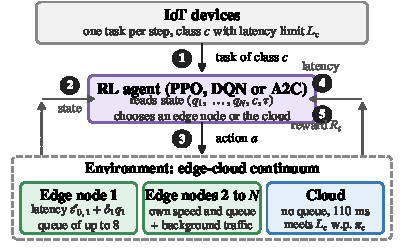
\includegraphics[width=0.95\columnwidth]{architecture.pdf}
\caption{Offloading loop. The numbers mark the steps of Section~\ref{sec:steps}.}
\label{fig:architecture}
\end{figure}

Edge node $i$ holds a queue of $q_i$ waiting tasks, with $0 \le q_i \le 8$. A task placed on edge node $i$ gets the latency
\begin{equation}
\ell = \ell_{0,i} + \delta_i\, q_i,
\label{eq:latency}
\end{equation}
where $\ell_{0,i}$ is the processing time of the node and $\delta_i$ is the extra wait for each task already in its queue. The latency is known when the task is placed, so a task on the edge meets its limit exactly when $\ell \le L_c$. The cloud has no queue. Its latency is 110\,ms on average, but the wide-area network makes it vary, so a cloud task of class $c$ meets its limit with a fixed probability $\pi_c$. In every system of this paper $\pi_c = 0$ for the most critical class, so the cloud never helps that class directly. Edge node $i$ finishes one task in a step with probability $d_i$. Other devices add background traffic that the agent does not control. Each background task joins the shortest edge queue. With $b$ background tasks per step on average, the offered edge load is
\begin{equation}
\rho = \frac{1 + b}{\sum_i d_i}.
\label{eq:load}
\end{equation}
All systems in this paper run at $\rho = 1$, so the edge can only keep up if some tasks go to the cloud and the classes compete for edge capacity. An episode has $T=200$ steps.

\begin{table}[t]
\caption{Symbols. Latencies in milliseconds.}
\label{tab:symbols}
\centering
\footnotesize
\setlength{\tabcolsep}{3pt}
\begin{tabular}{@{}l>{\raggedright\arraybackslash}p{6.2cm}@{}}
\toprule
Symbol & Meaning \\
\midrule
$N, K$ & number of edge nodes and of task classes \\
$c_t$ & class of the task at step $t$ \\
$p_c$ & share of tasks of class $c$ \\
$L_c$ & latency limit of class $c$ \\
$q_i$ & tasks waiting at edge node $i$, from 0 to 8 \\
$\ell_{0,i}, \delta_i$ & processing time of node $i$, wait per queued task \\
$d_i$ & chance that node $i$ finishes a task in a step \\
$\pi_c$ & chance that a cloud task of class $c$ meets its limit \\
$b$ & background tasks per step \\
$\rho$ & offered edge load, Eq.~\eqref{eq:load} \\
$T$, $\tau_t$ & steps per episode, share of the episode still to come \\
$w_c$ & miss penalty of class $c$ in the reward \\
$\bar w$ & miss penalty of the class-blind reward \\
$\beta, \kappa$ & reward for a met limit, cost of a cloud placement \\
$e_c$ & operator weight of a missed task of class $c$ \\
$v_c$ & share of tasks of class $c$ that miss the limit \\
$J$ & SLA cost per task, Eq.~\eqref{eq:cost} \\
\bottomrule
\end{tabular}
\end{table}

\subsection{Four Systems}
Table~\ref{tab:systems} lists the four systems. The nominal system is the one of the earlier conference version. It has two equal edge nodes and two classes, critical with a 50\,ms limit and analytics with a 90\,ms limit. An empty queue gives 30\,ms, which meets both limits. One waiting task gives 45\,ms, which still meets the critical limit. Two give 60\,ms, which misses the critical limit but meets the analytics limit. Background traffic arrives on a fixed schedule, one task every five steps, and the cloud never meets a limit. This makes the classes compete for the edge in the simplest possible way.

The three larger systems remove these simplifications. Their edge nodes differ in speed, background tasks arrive at random, and the cloud meets the analytics limit with some chance. Hetero3 has three edge nodes and two classes. Hetero3-3C has the same nodes and three classes with limits of 40, 70 and 110\,ms, which stand for control, interactive and analytics tasks. Large4-3C has four edge nodes and three classes. In the three-class systems the operator weights are 10, 4 and 1, and the cloud meets the 70\,ms limit with probability 0.2 and the 110\,ms limit with probability 0.6.

\begin{table}[t]
\caption{The four systems. All run at offered edge load $\rho=1$.}
\label{tab:systems}
\centering
\footnotesize
\setlength{\tabcolsep}{2.5pt}
\begin{tabular}{@{}lcccc@{}}
\toprule
 & Nominal & Hetero3 & Hetero3-3C & Large4-3C \\
\midrule
$N$, $K$ & 2, 2 & 3, 2 & 3, 3 & 4, 3 \\
$\ell_{0,i}$ & 30, 30 & 20, 30, 40 & 20, 30, 40 & 20, 25, 30, 40 \\
$\delta_i$ & 15, 15 & 10, 15, 20 & 10, 15, 20 & 10, 12, 15, 20 \\
$d_i$ & 0.6, 0.6 & 0.7, 0.6, 0.5 & 0.7, 0.6, 0.5 & 0.7, 0.6, 0.6, 0.5 \\
$b$, arrivals & 0.2, fixed & 0.8, random & 0.8, random & 1.4, random \\
$L_c$ & 50, 90 & 50, 90 & 40, 70, 110 & 40, 70, 110 \\
$p_c$ & 0.5, 0.5 & 0.5, 0.5 & 0.3, 0.3, 0.4 & 0.3, 0.3, 0.4 \\
$e_c$ & 10, 2 & 10, 2 & 10, 4, 1 & 10, 4, 1 \\
$\pi_c$ & 0, 0 & 0, 0.5 & 0, 0.2, 0.6 & 0, 0.2, 0.6 \\
States & 32,400 & 291,600 & 437,400 & 3,936,600 \\
\bottomrule
\end{tabular}
\end{table}

\subsection{Step by Step}
\label{sec:steps}
One step of the system runs as follows, numbered as in Fig.~\ref{fig:architecture}. (1) A device sends one task of class $c_t$. (2) The agent reads the state $s_t = (q_1,\dots,q_N, c_t, \tau_t)$, which holds the queue lengths, the class of the task and the share of the episode still to come, $\tau_t = 1 - t/T$. (3) The agent picks an action $a_t$, which is one of the edge nodes or the cloud. (4) The system computes the latency of the task from Eq.~\eqref{eq:latency}, or draws whether a cloud task meets its limit. If an edge node was chosen, the task joins its queue. Then the background tasks join the shortest queue, and each queue finishes one task with probability $d_i$. (5) The reward $R_t$ of Eq.~\eqref{eq:reward} is computed and used to update the agent. Then the next task arrives.

\subsection{Rewards}
With $m_t = 1$ if the task misses its limit and $m_t = 0$ otherwise, the reward of a step is
\begin{equation}
R_t = \beta\,(1-m_t) - w_{c_t}\, m_t - \kappa\,\mathbf{1}[a_t = \text{cloud}].
\label{eq:reward}
\end{equation}
A task that meets its limit earns $\beta = 1$. A task that misses costs $w_{c_t}$, the penalty of its class. The last term takes away $\kappa=0.1$ for every cloud placement, so the agent does not use the cloud without reason. Three choices of penalties are compared. The weighted reward uses the operator weights as penalties, $w_c = e_c$, which gives 10 and 2 in the nominal system. The class-blind (flat) reward uses one penalty for all classes,
\begin{equation}
\bar w = \sum_c p_c\, e_c ,
\label{eq:flat}
\end{equation}
which is 6 in the nominal system. Both rewards therefore have the same expected penalty for a missed task. The corrected reward is introduced in Section~\ref{sec:reward}. It has the same average penalty as the other two.

\subsection{Metrics and Objective}
For each class, $v_c$ is the share of tasks of that class that miss their limit. Edge use is the share of tasks placed on an edge node. One number is needed to rank policies. The SLA cost per task is
\begin{equation}
J = \sum_c p_c\, e_c\, v_c ,
\label{eq:cost}
\end{equation}
the expected operator weight of a missed task. In the nominal system $J = 5\,v_1 + v_2$, so a policy that misses every critical task and no analytics task has $J=5$. Because the weighted reward uses the operator weights as penalties, $J$ could seem to favor that reward by design. Section~\ref{sec:reward} shows that it does not favor it exactly, and the paper also reports the miss rate of every class, the full trade-off curve between the classes, and results for operator weights from 1:1 to 50:1.

\section{Exact Model}
\label{sec:exact}

Fig.~\ref{fig:overview} gives an overview of how the exact model is used. It computes the reference policies, tunes the rules, scores every trained agent, and gives the expected return that is used to choose hyperparameters.

\begin{figure*}[t]
\centering
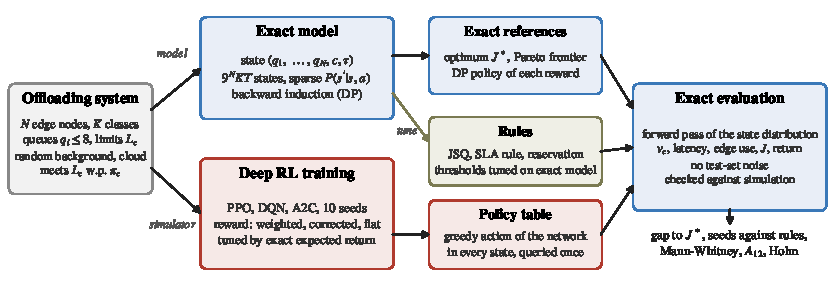
\includegraphics[width=\textwidth]{fig_overview.pdf}
\caption{Overview of the evaluation method. The exact model of each system gives the optimum, the Pareto frontier and the DP policy of each reward, and tunes the rules. Agents learn in the simulator only. Each trained network is turned into a table over all states and scored by the same exact forward pass as the rules and the DP policies.}
\label{fig:overview}
\end{figure*}

\subsection{The Observation Is the State}
In the nominal system the background schedule depends only on the step $t$, which the time share $\tau_t$ gives exactly. In the larger systems the background arrivals of each step are drawn independently of the past. In both cases the only random parts of a step are the service events, the background arrivals, the cloud outcome and the class of the next task, and all of them are independent of the history given the current queues and step. The observation $s_t$ is therefore a full description of the state, and each system is a finite-horizon Markov decision process \cite{puterman1994}. By the standard result for such processes, a deterministic policy that depends only on $s_t$ is optimal among all policies, including those that use the full history \cite{puterman1994}.

\subsection{Size and Transitions}
There are $9^N$ queue states, $K$ classes and $T=200$ steps, which gives the state counts of Table~\ref{tab:systems}. For a queue state and an action, the next queue state follows from three parts. The placed task joins its queue up to the cap of 8. The background tasks of the step join the shortest queue, with ties going to the lowest node index as in the simulator. Each non-empty queue then loses one task with probability $d_i$, independently of the others. This gives at most $2^N$ next queue states for each number of background tasks. The transitions are stored as one sparse matrix for each action and are built once. The class of the next task is drawn independently with probabilities $p_c$.

\subsection{Optimal Policies by DP}
Let $g(s,a)$ be the expected cost of action $a$ in state $s$, and let $P(s' \mid s,a)$ be the transition probability. Backward induction computes
\begin{equation}
V_t(s) = \min_{a} \Big[ g(s,a) + \sum_{s'} P(s' \mid s, a)\, V_{t+1}(s') \Big],
\label{eq:bellman}
\end{equation}
with $V_T = 0$, and the minimizing action gives the optimal policy at each step \cite{puterman1994}. With $g$ equal to $e_c$ times the chance of a miss, the expected total cost over an episode is $T$ times $J$, because the expected number of tasks of each class does not depend on the policy. The result is the policy with the lowest possible SLA cost, called the optimum. With $g = -\mathbb{E}[R_t]$ from Eq.~\eqref{eq:reward}, the result is the policy that a perfect learner of that reward would find, called the DP policy of the reward.

\subsection{Pareto Frontier}
For two classes, the paper solves Eq.~\eqref{eq:bellman} with $g$ equal to $\mu/p_1$ for a missed critical task and $(1-\mu)/p_2$ for a missed analytics task, for 101 values of $\mu$ between 0 and 1. Each solution minimizes $\mu\, v_1 + (1-\mu)\, v_2$. The resulting pairs of miss rates trace the lower boundary of all reachable pairs.

\subsection{Exact Evaluation of Any Policy}
For a deterministic policy given as a table over all states, the exact model starts from empty queues and propagates the probability of each state forward through the 200 steps. At each step it adds the expected misses, latency and edge placements of each class. Dividing by the expected number of tasks of each class gives the exact $v_c$, mean latencies, edge use and $J$. These are the values that a simulation with infinitely many episodes would give. A trained neural network is turned into such a table by asking it for its greedy action in every state once. The time share $\tau_t$ is computed with the same 32-bit numbers as in the simulator, so the table gives exactly the action that the network gives during a simulation. The same forward pass gives the exact expected return of a policy under any reward, which is used for hyperparameter selection in Section~\ref{sec:method}.

\subsection{Checks Against the Simulator}
The open test suite checks the exact model against the simulator. With the nominal parameters, the general simulator produces the same observations and rewards as the simulator of the conference version for 1,000 steps, and the general model gives the same optimal SLA cost as the earlier two-node model to within $10^{-12}$. In Hetero3 and Hetero3-3C, exact and simulated miss rates agree within one percentage point over 400 episodes for the optimum, and within 1.5 points for a random policy table, which is about three standard errors. Every transition matrix row sums to one, the optimum is never above any rule, and the exact expected return of a DP policy agrees with a 300-episode simulation within three standard errors.

\subsection{Cost of the Exact Solution}
Table~\ref{tab:scaling} shows how the exact solution grows with the number of edge nodes, for a homogeneous system with two classes at load 1 on one CPU core. Each extra node multiplies the queue states by 9 and the stored transitions by 14 to 24. Five nodes give 23.6 million states and need 16\,s to solve and 26\,s for one exact evaluation. A sixth node would again multiply the stored transitions by about 14, to roughly $1.6\times10^8$, which needs several gigabytes of memory. The exact benchmark is therefore a tool for systems of up to four or five nodes. A learned policy has a fixed size and decision time, whatever the number of nodes.

\begin{table}[t]
\caption{Size and time of the exact DP for $N$ equal edge nodes, two classes and load 1 (one CPU core).}
\label{tab:scaling}
\centering
\footnotesize
\setlength{\tabcolsep}{3pt}
\begin{tabular}{@{}rrrrrr@{}}
\toprule
$N$ & States & Transitions & Solve (s) & Evaluate (s) & Memory (MB) \\
\midrule
2 & 32,400 & 1,376 & 0.02 & 0.02 & 51 \\
3 & 291,600 & 32,050 & 0.19 & 0.08 & 53 \\
4 & 2,624,400 & 775,900 & 1.21 & 0.59 & 83 \\
5 & 23,619,600 & 11,302,060 & 15.71 & 25.89 & 477 \\
\bottomrule
\end{tabular}
\end{table}

\section{What Each Reward Optimizes}
\label{sec:reward}

\subsection{A Bonus Shifts Every Penalty}
The reward of Eq.~\eqref{eq:reward} gives $\beta$ for a met limit and $-w_c$ for a miss. Writing the reward of a missed task as $\beta - (w_c + \beta)$ shows that a miss costs $w_c + \beta$ relative to a met limit. This gives the following result.

\emph{Proposition 1.} For any policy, the expected total reward of an episode is
\begin{equation}
\mathbb{E}\Big[\sum_{t} R_t\Big] = T\beta - T\sum_c p_c\,(w_c + \beta)\, v_c - \kappa\, n_\text{cloud},
\label{eq:prop}
\end{equation}
where $n_\text{cloud}$ is the expected number of cloud placements. A policy maximizes the expected reward exactly when it minimizes $\sum_c p_c (w_c + \beta) v_c + \kappa\, n_\text{cloud}/T$.

\emph{Proof.} Each task gives $\beta - (w_{c_t} + \beta)\, m_t - \kappa\,\mathbf{1}[a_t=\text{cloud}]$. The expected number of tasks of class $c$ in an episode is $T p_c$ for every policy, because classes are drawn independently of the actions. The expected number of misses of class $c$ is therefore $T p_c v_c$, by the definition of $v_c$. Summing over the steps and taking expectations gives Eq.~\eqref{eq:prop}. The first term does not depend on the policy. \hfill$\blacksquare$

Three consequences follow. First, a learner of the weighted reward ranks misses by $w_c + \beta$, not by $w_c$. In the nominal system the penalties 10 and 2 act as 11 and 3, a ratio of 3.7 instead of the operator's 5. Second, the flat reward ranks all misses equally, so its optimal policy minimizes the overall miss rate plus the cloud term, whatever the operator weights are. Third, choosing
\begin{equation}
w_c = \alpha\, e_c - \beta, \qquad \alpha = \frac{\bar w + \beta}{\sum_c p_c e_c},
\label{eq:corrected}
\end{equation}
makes $w_c + \beta$ proportional to $e_c$ and keeps the average penalty at $\bar w$. This corrected reward ranks policies exactly as $J$ does, apart from the small cloud term. In the nominal system it gives penalties of 10.67 and 1.33. In the three-class systems it gives 11.17, 3.87 and 0.22, against weighted penalties of 10, 4 and 1. Proposition 1 holds for the undiscounted total reward. The learners of this paper use a discount factor below one, which the next subsection takes into account.

\subsection{Exact Consequences}
Table~\ref{tab:dprewards} gives the DP policy of each reward in each system. In the nominal system the weighted reward reaches an SLA cost of 0.2641, 1.0\% above the optimum of 0.2614, and the corrected reward reaches the optimum exactly. In Hetero3-3C the bonus moves the weighted reward 10.4\% above the optimum, while the corrected reward again reaches it. The flat reward is 65\% to 118\% above the optimum in every system. With a discount factor of 0.99, as used by the learners, the corrected reward stays within 0.8\% of the optimum in the first three systems and 4.1\% in Large4-3C. The flat reward gets worse with discounting in the larger systems, up to 174\% above the optimum.

\begin{table}[t]
\caption{Exact SLA cost of the optimum, and distance (\%) of the DP policy of each reward to it. W: weighted, C: corrected, F: flat. $\gamma$: discount factor of the DP policy.}
\label{tab:dprewards}
\centering
\footnotesize
\setlength{\tabcolsep}{2.6pt}
\begin{tabular}{@{}lccccccc@{}}
\toprule
 & & \multicolumn{3}{c}{$\gamma = 1$} & \multicolumn{3}{c}{$\gamma = 0.99$} \\
\cmidrule(lr){3-5} \cmidrule(l){6-8}
System & Optimum & W & C & F & W & C & F \\
\midrule
Nominal & 0.2614 & 1.0 & 0.0 & 95.2 & 3.3 & 0.0 & 95.2 \\
Hetero3 & 0.0899 & 1.1 & 0.1 & 64.6 & 1.7 & 0.8 & 115.5 \\
Hetero3-3C & 0.0839 & 10.4 & 0.0 & 116.2 & 10.5 & 0.1 & 169.7 \\
Large4-3C & 0.0777 & 4.9 & 0.1 & 118.2 & 5.5 & 4.1 & 174.0 \\
\bottomrule
\end{tabular}
\end{table}

Table~\ref{tab:ratios} changes the operator's weight ratio $e_1 : e_2$ in the nominal system from 1 to 50, with the average penalty fixed at 6. The flat reward is optimal only when the classes are equal. Its distance to the optimum grows from 17\% at a ratio of 2 to 95\% at 5 and 590\% at 50. The weighted reward stays within 1.5\% up to a ratio of 10, but reaches 8\% at 20 and 27\% at 50, because the bonus of 1 becomes large against the small analytics penalty. The corrected reward is optimal up to a ratio of 20 and 1\% above the optimum at 50, where the cloud term starts to matter. For ratios above 13, Eq.~\eqref{eq:corrected} gives a negative analytics penalty. This is still a valid reward. A missed analytics task then earns a small positive reward, which is less than the reward for a met limit, and only $w_c + \beta$ matters.

\begin{table}[t]
\caption{Operator weight ratio $e_1 : e_2$ in the nominal system, average penalty 6. SLA cost with weights $(e_1, e_2)$ scaled so that a ratio of 5 gives Eq.~\eqref{eq:cost}. Gap: distance of the DP policy of each reward to the optimum.}
\label{tab:ratios}
\centering
\footnotesize
\setlength{\tabcolsep}{2.5pt}
\begin{tabular}{@{}rccccc@{}}
\toprule
Ratio & Optimum & Corrected $w$ & Corrected & Weighted & Flat \\
\midrule
1 & 0.1021 & $6.00$, $6.00$ & 0.0\% & 0.0\% & 0.0\% \\
2 & 0.1746 & $8.33$, $3.67$ & 0.0\% & 0.2\% & 17.0\% \\
3 & 0.2128 & $9.50$, $2.50$ & 0.0\% & 0.8\% & 43.9\% \\
5 & 0.2614 & $10.67$, $1.33$ & 0.0\% & 1.0\% & 95.2\% \\
10 & 0.3435 & $11.73$, $0.27$ & 0.0\% & 1.5\% & 197.1\% \\
20 & 0.4743 & $12.33$, $-0.33$ & 0.0\% & 8.3\% & 330.3\% \\
50 & 0.7400 & $12.73$, $-0.73$ & 1.0\% & 26.9\% & 589.5\% \\
\bottomrule
\end{tabular}
\end{table}

\section{Agents, Baselines and Protocol}
\label{sec:method}

\subsection{Learning Agents and Tuning}
Three deep RL algorithms are trained. PPO \cite{schulman2017} and A2C \cite{mnih2016} learn a policy and a value function. DQN \cite{mnih2015} learns action values. All three come from Stable-Baselines3 \cite{raffin2021} and use the Gymnasium interface \cite{towers2024}. Agents are tested with their greedy action.

Every algorithm gets the same tuning budget, so that no reward or algorithm is helped by better settings. For each algorithm, six configurations are tried: the setting of the conference version and five drawn at random from a fixed grid (Table~\ref{tab:hyper}). For DQN the grid includes multiplying all rewards by 0.1, which does not change the optimal policy. Each configuration is trained with both the weighted and the flat reward, with two seeds (100 and 101) that are not used later, for 50,000 steps. The configuration with the highest exact expected return under its own reward is chosen. The SLA cost is never used for this choice, so the tuning does not favor the operator's objective. The corrected reward uses the setting chosen for the weighted reward.

\begin{table}[t]
\caption{Tuning grid and chosen settings. The same setting was chosen for both rewards for every algorithm. Unlisted settings are Stable-Baselines3 2.9.0 defaults.}
\label{tab:hyper}
\centering
\footnotesize
\setlength{\tabcolsep}{2.5pt}
\begin{tabular}{@{}l>{\raggedright\arraybackslash}p{3.6cm}l@{}}
\toprule
Algorithm & Grid & Chosen \\
\midrule
PPO & learning rate $\{1,3,10\}\times10^{-4}$, steps per update $\{512, 1024, 2048\}$, batch $\{64,128\}$, entropy $\{0, 0.01\}$, $\gamma$ $\{0.99, 0.999\}$, layers $\{2\times64, 2\times128\}$ & \shortstack[l]{lr $10^{-3}$, steps 1024\\batch 128, entropy 0.0\\$\gamma$ 0.99, layers $2\times128$} \\
\addlinespace
DQN & learning rate $\{1,3,10\}\times10^{-4}$, target update $\{500, 2000\}$, exploration share $\{0.1,0.3\}$, buffer $\{10^5,10^6\}$, $\gamma$ $\{0.99,0.999\}$, reward scale $\{1, 0.1\}$, layers $\{2\times64, 2\times128\}$ & \shortstack[l]{lr $10^{-4}$, $\gamma$ 0.99\\target 2000, expl. 0.1\\buffer $10^5$, scale 0.1\\layers $2\times128$} \\
\addlinespace
A2C & learning rate $\{3,7,10\}\times10^{-4}$, steps per update $\{5, 32, 128\}$, $\gamma$ $\{0.99,0.999\}$, entropy $\{0,0.01\}$, normalized advantage $\{\text{no},\text{yes}\}$, layers $\{2\times64, 2\times128\}$ & \shortstack[l]{lr $10^{-3}$, steps 5\\entropy 0.0, $\gamma$ 0.999\\norm. adv. no, layers $2\times128$} \\
\bottomrule
\end{tabular}
\end{table}

With the chosen settings, each agent is trained with 10 seeds, 0 to 9, for 100,000 steps in the nominal system. The exact model scores every agent every 5,000 steps, which gives learning curves without test noise. In the larger systems PPO is trained for 100,000 steps in Hetero3 and Hetero3-3C and 200,000 steps in Large4-3C, again with 10 seeds and all three rewards. Because the rules are tuned on the exact model of each system, PPO is tuned for each system too. The three PPO settings with the highest mean return in the nominal tuning are trained with both rewards, the two tuning seeds and the full budget of the system, and the one with the highest exact expected return is chosen. All 10-seed runs are also repeated with the nominal PPO setting.

\subsection{Rules}
Four rules serve as baselines, and two of them are tuned on the exact model of each system. Join-shortest-queue (JSQ) picks the edge node with the fewest waiting tasks and never uses the cloud. The SLA rule knows Eq.~\eqref{eq:latency} and every limit. It picks the edge node with the lowest predicted latency and uses it if that latency meets the limit of the task, and the cloud otherwise. The reservation rule adds one latency threshold for each class except the most critical one. A task of such a class goes to the edge only if the predicted latency of the best node is at most its threshold, which keeps capacity free for critical tasks. This is the form of the optimal admission policy for one pool of equal servers \cite{miller1969}. The thresholds are chosen by exhaustive search for two classes, and by coordinate search started from the SLA rule for three classes, minimizing the exact SLA cost. The reservation rule with node sets, called the node-set rule below, also lets each class use only a chosen subset of the edge nodes, for example only the slow nodes for analytics tasks. Subsets and thresholds are chosen by coordinate search on the exact model, started from the tuned reservation rule. All rules use the true latency model and the exact model of the system, which no learning agent sees. In the nominal system the node sets bring no gain, because the two nodes are equal.

\subsection{Published Reward Designs}
The flat reward is the design of Nieto et al. \cite{nieto2024}, in which the class is part of the state but every failed task has the same penalty. The design of Yamsani and Chenna Reddy \cite{yamsani2026} is rebuilt in three parts, following their equations. First, the penalty of class $c$ starts at $e_c$ and is updated after every task as $\lambda_c \leftarrow \max(0, \lambda_c + \eta\,(V_c - V^\ast))$, where $V_c$ is the miss rate of class $c$ over its last 200 tasks and $V^\ast = 0.05$ is their 95\% compliance target. Second, the state is extended with risk features that carry the same information as their risk score, which combines the expected latency against the deadline, the queue length and the recent miss history. The features are the predicted latency of each edge node divided by the limit of the task and the recent miss rate of each class. Third, following their pruning of clearly unsafe actions, edge nodes whose predicted latency misses the limit of the task are removed from the action set by invalid-action masking \cite{huang2022}. Their paper does not give the step size $\eta$, so two values are tested, 0.001 and 0.01. The agent is PPO with the tuned PPO setting, so that the comparison isolates the design and not the learner. A second version keeps only the adaptive penalties, without risk features and pruning. The full design uses features that are not part of the state of Section~\ref{sec:steps}, so it is scored by simulating 500 held-out episodes. All other agents are scored exactly.

\subsection{Changes of the System}
Five changes of the nominal system test what happens when the system differs from the one that rules and agents were built for. Tasks get slower, with 20\,ms instead of 15\,ms per waiting task. Service gets slower, with $d = 0.55$. Background traffic rises to 0.3 tasks per step. Background traffic becomes random with the same mean. The cloud meets the analytics limit with probability 0.5. For each change, four kinds of policies are scored exactly. The rules keep their nominal latency model and threshold. The trained PPO agents keep their nominal policy. The rules are tuned again with the true model of the changed system. The PPO agents are trained for another 25,000 steps in the changed system, starting from their nominal weights, which uses only interaction and rewards. The optimum of the changed system gives the reference.

\subsection{Statistics}
For learning agents the paper reports the mean over seeds with a 95\% bootstrap confidence interval from 10,000 resamples \cite{efron1993}. Rules and DP policies are deterministic and evaluated exactly, so they have no interval. Two groups of agents are compared with the two-sided Mann-Whitney U test \cite{mann1947}, which is exact when the samples have no tied values. The effect size is the Vargha-Delaney $A_{12}$ \cite{vargha2000}, the probability that a seed of the first group has a higher value than a seed of the second. Tests within one table are corrected with the Holm method \cite{holm1979}. Agents are compared with a deterministic rule by a two-sided sign test over seeds.

\section{Results}
\label{sec:results}

\subsection{Nominal System: Trained Agents (Q2, Q3)}
Table~\ref{tab:main} gives every policy in the nominal system after 100,000 training steps. PPO with the weighted reward misses 2.7\% of critical tasks and 15.4\% of analytics tasks, with an SLA cost of 0.287. This is 10\% above the optimum of 0.261. PPO with the flat reward misses 11.7\% of critical tasks and almost no analytics tasks, with an SLA cost of 0.588, which is 125\% above the optimum and close to the DP policy of the flat reward at 0.510. DQN shows the same pattern, with 0.339 for the weighted reward and 0.550 for the flat reward. Mean critical latency falls from 45.2\,ms to 36.7\,ms for PPO and from 44.8\,ms to 39.3\,ms for DQN. Every PPO and DQN agent sends at least 89\% of tasks to the edge, so none of them avoids misses by hiding tasks in the cloud.

\begin{table*}[t]
\caption{Nominal system after 100,000 training steps. Learning agents: mean over 10 seeds, with a 95\% bootstrap confidence interval for the SLA cost. Rules and DP policies: exact values. All values come from the exact model. Last column: seeds in which the agent has a lower SLA cost than the tuned reservation rule.}
\label{tab:main}
\centering
\footnotesize
\setlength{\tabcolsep}{3.2pt}
\begin{tabular}{@{}lccccccccc@{}}
\toprule
Policy & $v_1$ (\%) & $v_2$ (\%) & All (\%) & Lat. crit (ms) & Lat. ana (ms) & Edge (\%) & SLA cost $J$ & Above optimum & Beats rule \\
\midrule
JSQ & 51.8 & 14.4 & 33.1 & 61.5 & 61.5 & 100.0 & 2.735 & 946\% & \\
SLA rule & 11.7 & 0.0 & 5.8 & 45.4 & 39.7 & 94.2 & 0.583 & 123\% & \\
Reservation rule (tuned) & 1.3 & 24.1 & 12.7 & 34.4 & 49.3 & 87.3 & 0.304 & 16\% & \\
\midrule
A2C flat & 17.4 & 0.4 & 8.9 & 46.9 & 45.4 & 94.0 & 0.872 [0.678, 1.145] & 234\% & 0/10 \\
A2C weighted & 15.7 & 4.0 & 9.8 & 44.6 & 45.3 & 93.1 & 0.823 [0.614, 1.042] & 215\% & 0/10 \\
DQN flat & 11.0 & 0.2 & 5.6 & 44.8 & 44.0 & 94.5 & 0.550 [0.537, 0.569] & 111\% & 0/10 \\
DQN weighted & 4.8 & 10.1 & 7.4 & 39.3 & 44.4 & 92.6 & 0.339 [0.314, 0.361] & 30\% & 3/10 \\
PPO flat & 11.7 & 0.2 & 6.0 & 45.2 & 40.8 & 94.3 & 0.588 [0.562, 0.625] & 125\% & 0/10 \\
PPO weighted & 2.7 & 15.4 & 9.0 & 36.7 & 45.1 & 91.0 & 0.287 [0.279, 0.299] & 10\% & 9/10 \\
PPO corrected & 2.6 & 15.7 & 9.1 & 36.5 & 45.2 & 91.0 & 0.286 [0.279, 0.298] & 10\% & 9/10 \\
\midrule
DP flat & 10.2 & 0.0 & 5.1 & 44.3 & 46.6 & 94.9 & 0.510 & 95\% & \\
DP weighted & 2.4 & 14.3 & 8.3 & 37.4 & 46.4 & 91.7 & 0.264 & 1\% & \\
DP corrected & 2.1 & 15.8 & 8.9 & 36.9 & 46.6 & 91.1 & 0.261 & 0\% & \\
Optimum (DP) & 2.1 & 15.8 & 8.9 & 36.9 & 46.6 & 91.1 & 0.261 & 0\% & \\
\bottomrule
\end{tabular}
\end{table*}

Table~\ref{tab:tests} gives the statistics. For PPO and DQN, the weighted agent has fewer critical misses and a lower SLA cost than the flat agent with the same seed in all 10 seeds. The Vargha-Delaney effect size is 0.00 for both, which means that no weighted seed is above any flat seed. All of these differences stay significant after the Holm correction. The corrected reward does not differ from the weighted reward for PPO ($p=1.000$ after correction). Its DP policy is 1.0\% better, which is far below the spread between seeds after 100,000 steps. A2C, now tuned, learns a useful policy, but it is still far from the optimum and its two rewards do not differ in SLA cost.

\begin{table}[t]
\caption{Pairwise tests in the nominal system at 100,000 steps, 10 seeds each. Difference: first minus second reward, in percentage points for miss rates. $A_{12}$: chance that a seed of the first reward has a higher value. $p$: two-sided Mann-Whitney U test, Holm-corrected over all 15 rows. Last column: seeds in which the first reward is lower.}
\label{tab:tests}
\centering
\footnotesize
\setlength{\tabcolsep}{1.8pt}
\begin{tabular}{@{}llcrcrc@{}}
\toprule
Algo & Rewards & Metric & Diff. & $A_{12}$ & $p$ & Lower \\
\midrule
PPO & weighted vs flat & SLA cost & $-0.301$ & 0.00 & $<0.001$ & 10/10 \\
PPO & weighted vs flat & critical misses & $-9.1$ & 0.00 & $<0.001$ & 10/10 \\
PPO & weighted vs flat & analytics misses & $+15.2$ & 1.00 & $<0.001$ & 0/10 \\
PPO & corrected vs flat & SLA cost & $-0.302$ & 0.00 & $<0.001$ & 10/10 \\
PPO & corrected vs flat & critical misses & $-9.1$ & 0.00 & $<0.001$ & 10/10 \\
PPO & corrected vs flat & analytics misses & $+15.5$ & 1.00 & $<0.001$ & 0/10 \\
PPO & corrected vs weighted & SLA cost & $-0.001$ & 0.52 & 1.000 & 6/10 \\
PPO & corrected vs weighted & critical misses & $-0.1$ & 0.60 & 1.000 & 4/10 \\
PPO & corrected vs weighted & analytics misses & $+0.3$ & 0.47 & 1.000 & 5/10 \\
\midrule
DQN & weighted vs flat & SLA cost & $-0.212$ & 0.00 & $<0.001$ & 10/10 \\
DQN & weighted vs flat & critical misses & $-6.2$ & 0.00 & $<0.001$ & 10/10 \\
DQN & weighted vs flat & analytics misses & $+9.9$ & 1.00 & $<0.001$ & 0/10 \\
\midrule
A2C & weighted vs flat & SLA cost & $-0.049$ & 0.45 & 1.000 & 4/10 \\
A2C & weighted vs flat & critical misses & $-1.7$ & 0.39 & 1.000 & 6/10 \\
A2C & weighted vs flat & analytics misses & $+3.6$ & 0.96 & $<0.001$ & 0/10 \\
\bottomrule
\end{tabular}
\end{table}

The rules give the reference for Q3. JSQ never uses the cloud, so its queues fill up and it misses 51.8\% of critical tasks. The SLA rule knows the latency model and almost never misses an analytics task, but it misses 11.7\% of critical tasks, with an SLA cost of 0.583. Weighted PPO and weighted DQN beat it in all 10 seeds (sign test, $p=0.002$). The tuned reservation rule sends an analytics task to the edge only when a queue is empty. It misses 1.3\% of critical tasks and 24.1\% of analytics tasks, with an SLA cost of 0.304, which is 16\% above the optimum. Weighted PPO beats it in 9 of 10 seeds ($p=0.021$), and so does corrected PPO. Weighted DQN beats it in 3 of 10 seeds, which is not significant ($p=0.344$). With fair tuning and 100,000 steps, the best learned agent therefore beats a rule that knows the latency model and was tuned on the exact model.

Fig.~\ref{fig:frontier} places every agent against the optimal trade-off. The weighted and corrected PPO agents lie close to the frontier, near the optimum. The flat agents lie near the right end of the frontier, where almost no analytics tasks are missed. They are not bad policies in general. They give the lowest overall miss rate, 6.0\% for flat PPO against 9.0\% for weighted PPO, because the flat reward asks for exactly that, as Proposition 1 shows.

\begin{figure}[t]
\centering
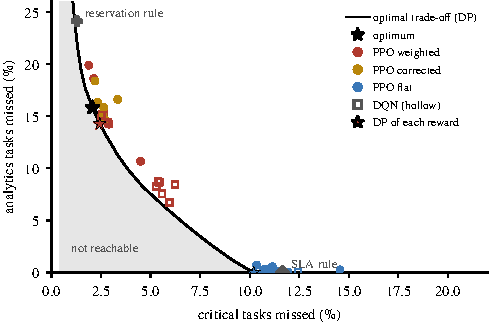
\includegraphics[width=\columnwidth]{fig_frontier_v3.pdf}
\caption{Trade-off between critical and analytics misses in the nominal system. The black line is the optimal trade-off from DP, and no policy can reach the gray area. Filled circles: PPO agents after 100,000 steps, one per seed. Hollow squares: DQN agents. Stars: the optimum and the DP policy of each reward.}
\label{fig:frontier}
\end{figure}

\subsection{Learning Curves and Training Budget}
Fig.~\ref{fig:curves} shows the SLA cost during training, scored exactly every 5,000 steps, over 10 seeds. Weighted PPO first reaches the level of the tuned reservation rule at 40,000 steps and stays at or below it for the rest of training, within 0.001. Corrected PPO reaches it at 50,000 steps and then moves around it. Flat PPO reaches about 0.57 after 20,000 steps and does not improve further. DQN with the scaled weighted reward reaches about 0.33 after 25,000 steps and stays between 0.31 and 0.35, so the instability of the conference settings is gone. A2C improves slowly and is still far from the other two at 100,000 steps. With the settings of the conference version and 20,000 steps, the reservation rule beat every agent in every seed. Both the tuning and the longer training are needed for the learned agents to reach the level of a tuned rule.

\begin{figure*}[t]
\centering
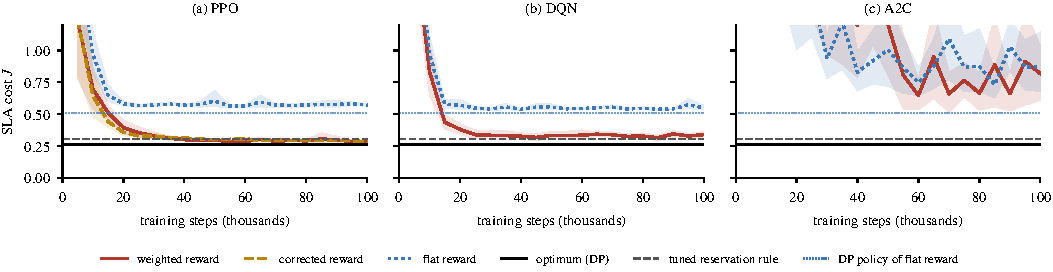
\includegraphics[width=\textwidth]{fig_curves_v3.pdf}
\caption{SLA cost during training in the nominal system, scored by the exact model every 5,000 steps. Mean over 10 seeds with 95\% bootstrap confidence interval. PPO updates in blocks of 1,024 steps, so its final policies in Table~\ref{tab:main} are taken after 100,352 steps, one update after the last point of the curve. Black line: optimum. Gray dashed line: tuned reservation rule. Thin dotted line: DP policy of the flat reward.}
\label{fig:curves}
\end{figure*}

\subsection{Published Reward Designs (Q3)}
Table~\ref{tab:pub} gives the design of Yamsani and Chenna Reddy \cite{yamsani2026} rebuilt in the nominal system. With risk features, action pruning and adaptive tiers, PPO reaches an SLA cost of 0.368 with a step size of 0.001 and 0.418 with 0.01, which is 41\% and 60\% above the optimum. With adaptive tiers alone it reaches 0.414. All three versions are better than the flat reward of Nieto et al. \cite{nieto2024} in every seed, and worse than the fixed weighted reward in every seed (Mann-Whitney, $p<0.001$ for each comparison). None of them beats the tuned reservation rule in any seed.

\begin{table}[t]
\caption{Rebuilt design of Yamsani and Chenna Reddy \cite{yamsani2026} in the nominal system, PPO, 100,000 steps, 10 seeds. Penalties: mean penalty of the critical and the analytics tier at the end of training. The full design is scored by 500 simulated episodes, because its state has risk features (standard error of each SLA cost below 0.01). All other rows are exact.}
\label{tab:pub}
\centering
\footnotesize
\setlength{\tabcolsep}{2pt}
\begin{tabular}{@{}lccccc@{}}
\toprule
Variant & $\eta$ & SLA cost $J$ & Above & $v_1$ (\%) & Penalties \\
\midrule
full design & 0.001 & 0.368 [0.346, 0.393] & 41\% & 5.9 & 11.1, 4.7 \\
full design & 0.01 & 0.418 [0.380, 0.453] & 60\% & 7.3 & 30.0, 14.1 \\
adaptive tiers only & 0.01 & 0.414 [0.396, 0.434] & 58\% & 7.1 & 38.1, 23.1 \\
\midrule
PPO weighted & & 0.287 [0.279, 0.299] & 10\% & 2.7 & 10, 2 \\
PPO flat & & 0.588 [0.562, 0.625] & 125\% & 11.7 & 6, 6 \\
\bottomrule
\end{tabular}
\end{table}

Proposition 1 explains the result. The design raises the penalty of a tier whenever its recent miss rate is above the target of 5\%. In this system the optimum misses 15.8\% of analytics tasks, so the analytics target cannot be met together with a low critical miss rate. Both penalties keep growing, and the analytics penalty grows faster relative to its start. After training the penalties are 11.1 and 4.7 with the smaller step size, and 30.0 and 14.1 with the larger one. With the bonus of 1, they act as a ratio of about 2:1 instead of the operator's 5:1, so the agent moves toward the class-blind policy. Adaptive penalties work well when every target is reachable \cite{altman1999,tessler2019}. When the targets are set without knowing what is possible, they can undo the per-class weighting that the tiers were meant to provide. The exact model shows which targets are reachable, through the Pareto frontier of Fig.~\ref{fig:frontier}.

\subsection{Larger Systems (Q4)}
Table~\ref{tab:scen} and Fig.~\ref{fig:scen} give the three larger systems. PPO was tuned again for each system with the same protocol, now with the three best PPO settings of the nominal tuning, two tuning seeds and the full budget. The default setting was chosen for Hetero3 and Large4-3C, and the nominal setting for Hetero3-3C. The rules are much further from the optimum here than in the nominal system. The tuned reservation rule is 32\% to 89\% above the optimum, and the rule with node sets 21\% to 31\%.

\begin{table}[t]
\caption{Larger systems. PPO tuned for each system, mean over 10 seeds with 95\% bootstrap interval. Rules: exact. Miss rates per class in \%. Last column: seeds in which PPO beats the node-set rule.}
\label{tab:scen}
\centering
\footnotesize
\setlength{\tabcolsep}{1.6pt}
\begin{tabular}{@{}lcccc@{}}
\toprule
Policy & SLA cost $J$ & Above opt. & $v_c$ (\%) & Beats \\
\midrule
\multicolumn{5}{@{}l}{\emph{Hetero3}, optimum 0.0899} \\
\quad SLA rule & 0.527 & 486\% & 10.5, 0.0 & \\
\quad Reservation rule & 0.141 & 57\% & 1.3, 7.6 & \\
\quad Node-set rule & 0.117 & 31\% & 0.6, 8.9 & \\
\quad PPO flat & 0.158 [0.147, 0.169] & 75\% & 2.2, 4.9 & 0/10 \\
\quad PPO weighted & 0.129 [0.116, 0.144] & 43\% & 1.1, 7.6 & 4/10 \\
\quad PPO corrected & 0.123 [0.116, 0.130] & 36\% & 0.7, 8.7 & 2/10 \\
\addlinespace
\multicolumn{5}{@{}l}{\emph{Hetero3-3C}, optimum 0.0839} \\
\quad SLA rule & 0.697 & 731\% & 23.2, 0.2, 0.0 & \\
\quad Reservation rule & 0.158 & 89\% & 1.5, 0.5, 27.0 & \\
\quad Node-set rule & 0.110 & 31\% & 1.8, 0.6, 12.3 & \\
\quad PPO flat & 0.298 [0.253, 0.346] & 255\% & 8.0, 3.6, 3.5 & 0/10 \\
\quad PPO weighted & 0.140 [0.130, 0.151] & 67\% & 2.5, 1.8, 10.9 & 0/10 \\
\quad PPO corrected & 0.140 [0.125, 0.161] & 67\% & 2.6, 1.0, 12.1 & 0/10 \\
\addlinespace
\multicolumn{5}{@{}l}{\emph{Large4-3C}, optimum 0.0777} \\
\quad SLA rule & 0.511 & 557\% & 17.0, 0.1, 0.0 & \\
\quad Reservation rule & 0.102 & 32\% & 1.0, 0.2, 17.3 & \\
\quad Node-set rule & 0.094 & 21\% & 1.1, 0.5, 13.9 & \\
\quad PPO flat & 0.340 [0.300, 0.382] & 338\% & 9.3, 4.5, 2.0 & 0/10 \\
\quad PPO weighted & 0.125 [0.119, 0.133] & 61\% & 2.1, 1.7, 10.8 & 0/10 \\
\quad PPO corrected & 0.120 [0.116, 0.123] & 54\% & 1.9, 1.1, 12.2 & 0/10 \\
\bottomrule
\end{tabular}
\end{table}

\begin{figure*}[t]
\centering
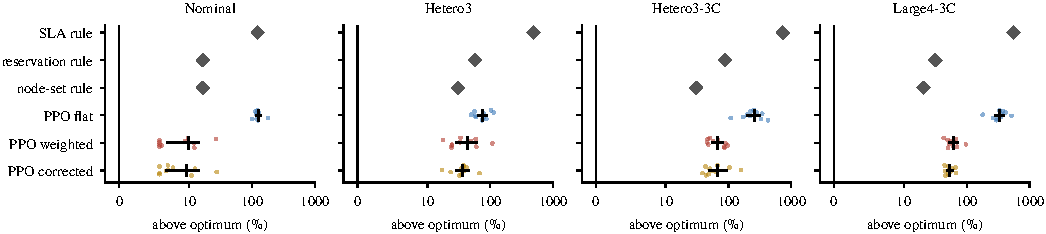
\includegraphics[width=\textwidth]{fig_scenarios_v3.pdf}
\caption{Distance of every policy to the optimum of its system, in percent on a scale that is linear below 10\% and logarithmic above. Diamonds: rules, exact. Dots: PPO agents, one per seed, with the mean and its 95\% bootstrap interval in black. Nominal system after 100,000 steps, Hetero3 and Hetero3-3C after 100,000 steps, Large4-3C after 200,000 steps.}
\label{fig:scen}
\end{figure*}

The effect of the reward carries over to every larger system. The weighted reward lowers the SLA cost of PPO against the flat reward in Hetero3 from 0.158 to 0.129, in Hetero3-3C from 0.298 to 0.140 and in Large4-3C from 0.340 to 0.125. All three differences are significant after the Holm correction ($p \le 0.036$), and in the three-class systems every weighted seed is below every flat seed. The corrected reward gives 0.123, 0.140 and 0.120, which does not differ significantly from the weighted reward in any system. Its exact advantage of up to 10\% in the DP policies is therefore smaller than what PPO reaches in practice.

The trained agents are still far from the optimum, 36\% to 67\% above it for the weighted and corrected rewards. They beat the SLA rule in every seed of every system. Against the tuned reservation rule the picture depends on the system. Corrected PPO beats it in 9 of 10 seeds in Hetero3 ($p=0.021$), weighted and corrected PPO beat it in 8 of 10 seeds in Hetero3-3C ($p=0.109$), and no agent beats it in Large4-3C. The rule with node sets is better than every agent in Hetero3-3C and Large4-3C, and better than most seeds in Hetero3. In these systems a rule that knows the latency model and is tuned on the exact model is still the stronger choice. The agents learn from rewards alone and reach this level without any model, but the exact benchmark shows that they leave a large part of the possible gain unused.

With the nominal PPO setting instead of the setting tuned per system, the weighted reward reaches 0.134, 0.140 and 0.162, and the corrected reward 0.117, 0.140 and 0.133. The order of the rewards is the same. The setting matters most in Large4-3C, where the default setting is more stable across seeds and lowers the cost of weighted PPO from 0.162 to 0.125. In Hetero3 the nominal setting is slightly better for the corrected reward, which then beats the node-set rule in 7 of 10 seeds.

\subsection{Changes of the System (Q5)}
Table~\ref{tab:shift} and Fig.~\ref{fig:shift} give the five changes of the nominal system. Every value is the distance to the optimum of the changed system. The SLA rule with the nominal latency model is 106\% to 239\% above the optimum. The tuned reservation rule keeps its nominal threshold, which sends an analytics task to the edge only when a queue is empty. Tuning it again with the true model of the changed system picks the same threshold in all five cases, so the rule loses nothing from the change and stays 6\% to 16\% above the optimum. This matches the structure of the optimal policy for one pool of servers \cite{miller1969}, which does not depend on the exact speeds.

\begin{table*}[t]
\caption{Changes of the nominal system. Distance of the SLA cost to the optimum of the changed system, exact. Nominal: policy or threshold of the nominal system used unchanged. Re-tuned: thresholds chosen again on the exact model of the changed system. Fine-tuned: nominal PPO network trained for another 25,000 steps in the changed system. PPO values are means over 10 seeds.}
\label{tab:shift}
\centering
\footnotesize
\setlength{\tabcolsep}{4pt}
\begin{tabular}{@{}lcccccccc@{}}
\toprule
 & & SLA rule & \multicolumn{2}{c}{Reservation rule} & \multicolumn{2}{c}{PPO weighted} & \multicolumn{2}{c}{PPO flat} \\
\cmidrule(lr){4-5} \cmidrule(lr){6-7} \cmidrule(l){8-9}
Change & Optimum & nominal model & nominal & re-tuned & nominal & fine-tuned & nominal & fine-tuned \\
\midrule
slower tasks & 0.261 & 123\% & 16\% & 16\% & 10\% & 10\% & 127\% & 120\% \\
slower service & 0.442 & 163\% & 6\% & 6\% & 14\% & 14\% & 166\% & 158\% \\
more background & 0.427 & 168\% & 6\% & 6\% & 15\% & 12\% & 172\% & 167\% \\
random background & 0.341 & 106\% & 6\% & 6\% & 4\% & 5\% & 107\% & 99\% \\
cloud meets analytics limit w.p. 0.5 & 0.172 & 239\% & 7\% & 7\% & 22\% & 19\% & 242\% & 234\% \\
\bottomrule
\end{tabular}
\end{table*}

\begin{figure}[t]
\centering
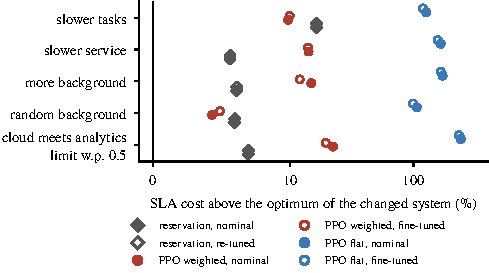
\includegraphics[width=\columnwidth]{fig_shift_v3.pdf}
\caption{Distance to the optimum of the changed system for the reservation rule and PPO, on a scale that is linear below 10\% and logarithmic above. Filled markers: nominal rule or policy used unchanged. Hollow markers: re-tuned rule or fine-tuned agent. PPO values are means over 10 seeds.}
\label{fig:shift}
\end{figure}

The trained PPO agents also keep most of their quality without any new training. Weighted PPO with its nominal policy is 4\% to 22\% above the new optimum. It beats the unchanged reservation rule in 9 of 10 seeds when tasks get slower and when the background becomes random, and loses to it under the other three changes. Another 25,000 steps of training in the changed system move the weighted agents by at most 3 percentage points, to between 5\% and 19\% above the optimum. The order of the rewards does not change. Flat PPO is 99\% to 242\% above the optimum under every change, with or without fine-tuning. In these changes the best structure stays the same, which is to keep the edge free for critical tasks, so a policy that has learned this structure keeps working.

\subsection{Sensitivity at a Short Budget}
The conference version also changed the penalty ratio, the load, the class mix and the learning rate, with PPO in its default setting, 20,000 steps and 10 seeds (5 for the learning rate). These results are scored with the exact model and summarized here. Fig.~\ref{fig:sweeps}(a) changes the penalty ratio with the average penalty fixed at 6. Critical misses fall from 13.6\% at 6:6 to 5.1\% at 11:1, and analytics misses rise from 0.8\% to 19.5\%. Fig.~\ref{fig:sweeps}(b) changes the service probability $d$ from 0.9 to 0.5, which moves the offered load from 0.67 to 1.2. With spare capacity, at a load of 0.67 and 0.75, both rewards miss almost no tasks and do not differ ($p=0.940$ and $p=0.853$). At a load of 1.2 the weighted reward halves the SLA cost of the flat reward, 1.099 against 2.112 ($p<0.001$). The per-class penalty matters only when the classes compete for the edge. Fig.~\ref{fig:sweeps}(c) changes the share of critical tasks. At 30\% critical tasks the weighted reward lowers the SLA cost from 0.785 to 0.537 ($p=0.005$). At 70\% it lowers the mean from 0.894 to 0.633, which is not significant ($p=0.105$). A learning rate of $10^{-4}$ does not learn within 20,000 steps with either reward. At $3\times10^{-4}$ and $10^{-3}$ the weighted reward has the lower SLA cost.

\begin{figure*}[t]
\centering
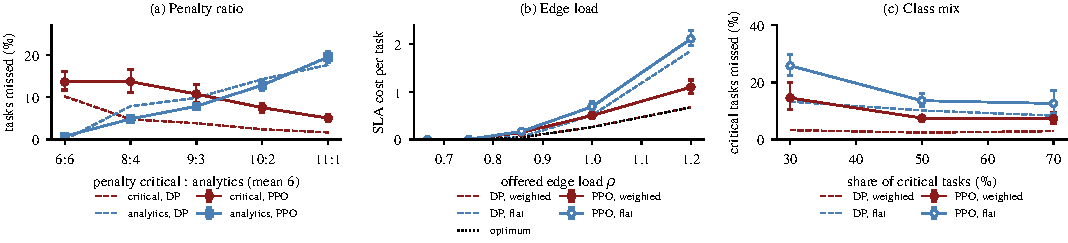
\includegraphics[width=\textwidth]{fig_sweeps.pdf}
\caption{Sensitivity of PPO with the conference setting at 20,000 steps, mean over 10 seeds with 95\% bootstrap confidence interval, against the DP policy for the same reward (dashed). (a) Penalty ratio with the average penalty fixed at 6. (b) Offered edge load $\rho$, changed through the service probability $d$. (c) Share of critical tasks, with the flat penalty matched to the mix by Eq.~\eqref{eq:flat}.}
\label{fig:sweeps}
\end{figure*}

\subsection{Short Test Sets}
Every agent was also simulated on 100 held-out episodes. Short and fixed test sets can move results noticeably. Table~\ref{tab:protocol} shows the critical miss rate of three fixed policies, exact and simulated. With the 20 episodes used in the conference version, the SLA rule shows 10.67\% critical misses against an exact 11.65\%. With 3,000 episodes the difference falls below 0.1 percentage points. A shift of one percentage point is as large as some of the differences that offloading papers report, which is why every number in this paper comes from the exact model.

\begin{table}[t]
\caption{Critical miss rate (\%) of three fixed policies in the nominal system, exact and simulated on fixed test sets of different size.}
\label{tab:protocol}
\centering
\footnotesize
\setlength{\tabcolsep}{4pt}
\begin{tabular}{@{}lcccc@{}}
\toprule
Policy & Exact & 20 episodes & 100 episodes & 3,000 episodes \\
\midrule
SLA rule & 11.65 & 10.67 & 12.59 & 11.72 \\
Reservation rule & 1.26 & 1.01 & 1.39 & 1.29 \\
Optimum (DP) & 2.06 & 1.71 & 2.25 & 2.09 \\
\bottomrule
\end{tabular}
\end{table}

\section{Discussion}
\label{sec:discussion}

\subsection{What the Results Show}
The per-class penalty is the part of the reward that decides which tasks are protected. Proposition 1 shows why. A learner maximizes the expected reward, which is the same as minimizing the sum of $(w_c + \beta)$ times the misses of each class. With one penalty for all classes, this is the overall miss rate, and the DP policy of the flat reward is 65\% to 118\% above the optimum in every system, however well it is learned. With the operator weights as penalties, the reward is close to the operator's objective, and with the corrected penalties of Eq.~\eqref{eq:corrected} it is the operator's objective. Trained PPO agents follow the same order in every system, and DQN agents in the nominal system.

The exact benchmark also shows how much the learners leave on the table. In the nominal system the best agent is 10\% above the optimum and beats a tuned rule. In the larger systems the agents are 36\% to 67\% above the optimum. They beat the simple reservation rule in two of the three systems, but the node-set rule, which knows the latency model and is tuned on the exact model, is better in all three. Without an optimal reference, an agent that beats join-shortest-queue, an SLA rule and a class-blind version of itself would look strong in all four systems. The gap to the optimum would stay invisible.

The rebuilt published design points to the same cause from another side. Its adaptive tiers raise every penalty whose target is missed. When the targets cannot all be met, the penalties drift toward each other, and the agent drifts toward the class-blind policy. In the nominal system this left it 41\% to 60\% above the optimum, between the fixed weighted reward and the flat reward. Setting penalty targets is safe only when it is known which targets are reachable, which the exact frontier shows.

\subsection{When to Use Which Policy}
If the latency model is known and the system is small enough for the exact model, the DP policy is the best choice, because it is optimal by construction. A tuned reservation rule is a good second choice. It needs only the latency model and a search over a few thresholds, and under every change of the nominal system that was tested it stayed between 6\% and 16\% above the new optimum without being tuned again. A learned agent is useful when the latency model is not known or changes, or when the system is too large for the exact model. Table~\ref{tab:scaling} shows that this happens quickly, since every extra edge node multiplies the stored transitions of the exact model by 14 to 24. In that case the results of this paper give three practical rules. Use a per-class penalty, because a class-blind penalty optimizes the wrong objective. Fold the bonus for a met limit into the penalties with Eq.~\eqref{eq:corrected}, so that the reward has the operator's weights. Tune and train long enough, and check the result against a strong rule.

\subsection{Threats to Validity}
The systems are synthetic. Latencies follow a linear queue model, the cloud is described only by the chance to meet each limit, and there is no energy or transmission model. Real traces were not available to the authors. The results show what the reward does in systems where the answer can be checked exactly, not how large the effect is in a deployed system. The SLA cost uses the operator weights, which the weighted reward also uses. The per-class miss rates, the trade-off curve of Fig.~\ref{fig:frontier} and the weight sweep of Table~\ref{tab:ratios} let a reader with other weights judge every policy. The agents use standard multilayer networks from one library, tuned with six configurations in the nominal system and three in each larger system. Other architectures, longer training or larger searches could bring them closer to the optimum. The rebuilt published design follows the equations of its paper, but parameters the paper does not give had to be chosen, and two step sizes were tested for that reason. All exact values rely on the exact model, which the test suite checks against the simulator.

\section{Conclusion}
\label{sec:conclusion}

This paper studied the reward of deep RL task offloading in the IoT edge-cloud continuum against an exact optimum. Four systems with up to four heterogeneous edge nodes and three task classes were solved by DP, which gave the optimal policy, the optimal trade-off between the classes and an exact score for every trained agent. A reward with a bonus for a met limit ranks policies by the per-class penalty plus the bonus. A class-blind penalty therefore minimizes the overall miss rate and stays 65\% to 118\% above the optimum with a perfect learner, while a corrected per-class penalty reaches the optimum. Trained PPO agents show the same effect in every system and DQN agents in the nominal system, and in the nominal system tuned PPO comes within 10\% of the optimum and beats a tuned reservation rule in 9 of 10 seeds. In the larger systems the agents remain 36\% to 67\% above the optimum, and a node-set rule tuned on the exact model is better than every agent. A rebuilt published design with adaptive penalty tiers stays between the weighted and the class-blind reward, because its targets cannot all be met and its penalties drift together. Future work will use the exact benchmark to test learners that use the structure of the system, approximate DP for systems beyond five edge nodes, and models of energy and transmission as in \cite{hu2021,zhang2024}.


\begin{thebibliography}{00}
\bibitem{mao2017} Y. Mao, C. You, J. Zhang, K. Huang, and K. B. Letaief, ``A survey on mobile edge computing: The communication perspective,'' \emph{IEEE Commun. Surveys Tuts.}, vol. 19, no. 4, pp. 2322--2358, 2017.
\bibitem{mnih2015} V. Mnih \emph{et al.}, ``Human-level control through deep reinforcement learning,'' \emph{Nature}, vol. 518, pp. 529--533, 2015.
\bibitem{sutton2018} R. S. Sutton and A. G. Barto, \emph{Reinforcement Learning: An Introduction}, 2nd ed. Cambridge, MA, USA: MIT Press, 2018.
\bibitem{hu2021} J. Hu, Y. Li, G. Zhao, B. Xu, Y. Ni, and H. Zhao, ``Deep reinforcement learning for task offloading in edge computing assisted power IoT,'' \emph{IEEE Access}, vol. 9, pp. 93892--93901, 2021.
\bibitem{chen2025} Z. Chen and W. Li, ``Optimization of task offloading using deep reinforcement learning in wireless power transfer and edge computing systems,'' in \emph{Proc. Int. Conf. Sensor-Cloud Edge Comput. Syst. (SCECS)}, 2025, pp. 9--13.
\bibitem{zhang2024} T. Zhang, D. Xu, A. Tolba, K. Yu, H. Song, and S. Yu, ``Reinforcement-learning-based offloading for RIS-aided cloud-edge computing in IoT networks: Modeling, analysis, and optimization,'' \emph{IEEE Internet Things J.}, vol. 11, no. 11, pp. 19421--19439, 2024.
\bibitem{alqerm2021} I. AlQerm and J. Pan, ``DeepEdge: A new QoE-based resource allocation framework using deep reinforcement learning for future heterogeneous Edge-IoT applications,'' \emph{IEEE Trans. Netw. Service Manag.}, vol. 18, no. 4, pp. 3942--3954, 2021.
\bibitem{heidari2023} A. Heidari, M. A. J. Jamali, N. J. Navimipour, and S. Akbarpour, ``A QoS-aware technique for computation offloading in IoT-edge platforms using a convolutional neural network and Markov decision process,'' \emph{IT Prof.}, vol. 25, no. 1, pp. 24--39, 2023.
\bibitem{nieto2024} G. Nieto, I. de la Iglesia, U. Lopez-Novoa, and C. Perfecto, ``Deep reinforcement learning techniques for dynamic task offloading in the 5G edge-cloud continuum,'' \emph{J. Cloud Comput.}, vol. 13, art. 94, 2024.
\bibitem{lan2024} S. Lan \emph{et al.}, ``SLA-ORECS: An SLA-oriented framework for reallocating resources in edge-cloud systems,'' \emph{J. Cloud Comput.}, vol. 13, art. 18, 2024.
\bibitem{yamsani2026} N. Yamsani and P. Chenna Reddy, ``SLA aware deep reinforcement learning for adaptive EdgeCloud task scheduling,'' \emph{Sci. Rep.}, vol. 16, art. 10037, 2026.
\bibitem{puterman1994} M. L. Puterman, \emph{Markov Decision Processes: Discrete Stochastic Dynamic Programming}. New York, NY, USA: Wiley, 1994.
\bibitem{henderson2018} P. Henderson, R. Islam, P. Bachman, J. Pineau, D. Precup, and D. Meger, ``Deep reinforcement learning that matters,'' in \emph{Proc. AAAI Conf. Artif. Intell.}, vol. 32, no. 1, 2018.
\bibitem{agarwal2021} R. Agarwal, M. Schwarzer, P. S. Castro, A. C. Courville, and M. G. Bellemare, ``Deep reinforcement learning at the edge of the statistical precipice,'' in \emph{Proc. Adv. Neural Inf. Process. Syst. (NeurIPS)}, vol. 34, 2021, pp. 29304--29320.
\bibitem{ng1999} A. Y. Ng, D. Harada, and S. Russell, ``Policy invariance under reward transformations: Theory and application to reward shaping,'' in \emph{Proc. 16th Int. Conf. Mach. Learn. (ICML)}, 1999, pp. 278--287.
\bibitem{altman1999} E. Altman, \emph{Constrained Markov Decision Processes}. Boca Raton, FL, USA: Chapman \& Hall/CRC, 1999.
\bibitem{tessler2019} C. Tessler, D. J. Mankowitz, and S. Mannor, ``Reward constrained policy optimization,'' in \emph{Proc. Int. Conf. Learn. Represent. (ICLR)}, 2019.
\bibitem{miller1969} B. L. Miller, ``A queueing reward system with several customer classes,'' \emph{Manage. Sci.}, vol. 16, no. 3, pp. 234--245, 1969.
\bibitem{huang2022} S. Huang and S. Onta\~n\'on, ``A closer look at invalid action masking in policy gradient algorithms,'' in \emph{Proc. Int. FLAIRS Conf.}, vol. 35, 2022.
\bibitem{schulman2017} J. Schulman, F. Wolski, P. Dhariwal, A. Radford, and O. Klimov, ``Proximal policy optimization algorithms,'' \emph{arXiv:1707.06347}, 2017.
\bibitem{mnih2016} V. Mnih \emph{et al.}, ``Asynchronous methods for deep reinforcement learning,'' in \emph{Proc. 33rd Int. Conf. Mach. Learn. (ICML)}, 2016, pp. 1928--1937.
\bibitem{raffin2021} A. Raffin, A. Hill, A. Gleave, A. Kanervisto, M. Ernestus, and N. Dormann, ``Stable-Baselines3: Reliable reinforcement learning implementations,'' \emph{J. Mach. Learn. Res.}, vol. 22, no. 268, pp. 1--8, 2021.
\bibitem{towers2024} M. Towers \emph{et al.}, ``Gymnasium: A standardized interface for reinforcement learning environments,'' \emph{arXiv:2407.17032}, 2024.
\bibitem{efron1993} B. Efron and R. J. Tibshirani, \emph{An Introduction to the Bootstrap}. New York, NY, USA: Chapman \& Hall, 1993.
\bibitem{mann1947} H. B. Mann and D. R. Whitney, ``On a test of whether one of two random variables is stochastically larger than the other,'' \emph{Ann. Math. Statist.}, vol. 18, no. 1, pp. 50--60, 1947.
\bibitem{vargha2000} A. Vargha and H. D. Delaney, ``A critique and improvement of the CL common language effect size statistics of McGraw and Wong,'' \emph{J. Educ. Behav. Statist.}, vol. 25, no. 2, pp. 101--132, 2000.
\bibitem{holm1979} S. Holm, ``A simple sequentially rejective multiple test procedure,'' \emph{Scand. J. Statist.}, vol. 6, no. 2, pp. 65--70, 1979.
\end{thebibliography}

\end{document}
